
\begin{frame}[c]
  \frametitle{Case VI : Waste Package Failure Time and Diffusion Coefficient}

The time of waste package failure was not expected to greatly effect the 
magnitude of the mean of the peak doses except for cases in which waste package failure times 
exceeded the half lives of dominant dose-contributing nuclides. 
That is, since the dominant dose-contributing 
radionuclides for the reference case are quite long lived ($^{129}I$, etc.), 
all but the longest reasonable waste package containment lifetime is overwhelmed by 
the half life of the dominant radionuclides. The long time scales of 
radionuclide release was expected to render the the waste package lifetime 
irrelevant if it was shorter than a million years. 
\end{frame}

\begin{frame}[c]
  \frametitle{Case VI : Waste Package Failure Time and Diffusion Coefficient}
Though the model contains a unit cell-type model, it is possible to determine, 
in post processing, the results of a simulation with temporally heterogeneous 
failures among waste packages. That is, by a weighted sum of the time histories 
of the no-fail case and the all-fail case, it is possible to mimic a 
time-varying failure among the many waste packages. 

\end{frame}

\begin{frame}[c]
  \frametitle{Case VI : Waste Package Failure Time and Diffusion Coefficient}

To investigate the effect of the waste package failure time, it was varied over 
five magnitudes from one thousand to ten million years. Simultaneously, the reference 
diffusivity was varied over the eight magnitudes between $1\times10^{-8}$ and 
$1\times10^{-15}$ in order to determine the correlation between increased 
radionuclide mobility and the waste package lifetime. 

\end{frame}

\begin{frame}[c]
  \frametitle{Case VI : Waste Package Failure Time and Diffusion Coefficient}

For the clay repository, the waste package failure time is entirely irrelevant 
until waste package failure times reach the million or ten million year time 
scale. 

\begin{figure}[ht!]
\centering
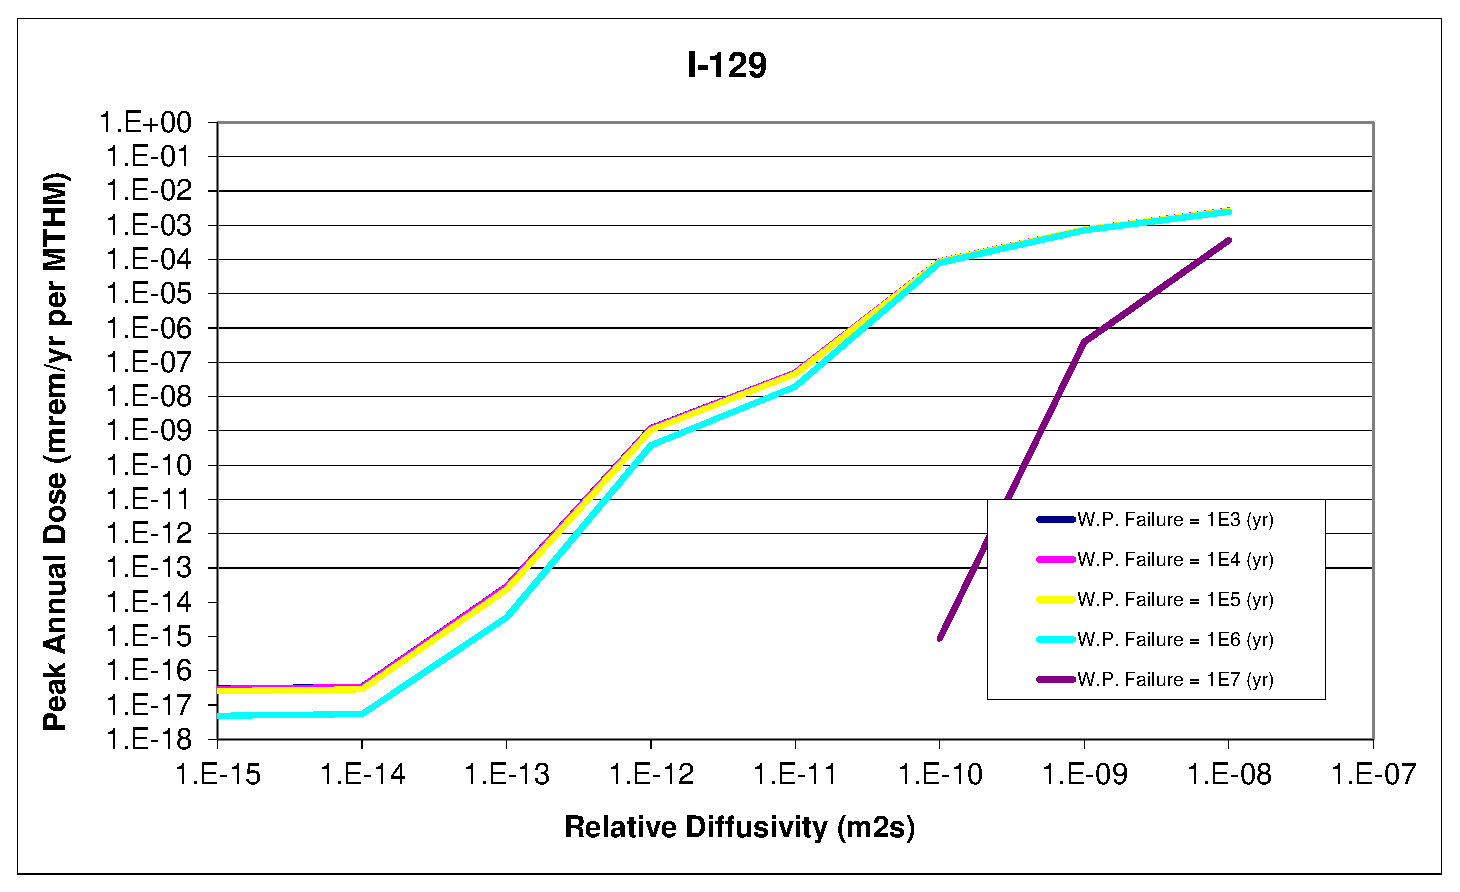
\includegraphics[width=0.8\textwidth]{WPFailExtended/I-129.eps}
\caption{$^{129}I$ waste package failure time sensitivity. }
\label{fig:WPFailI129}
\end{figure}
\end{frame}

\begin{frame}[c]
  \frametitle{Case VI : Waste Package Failure Time and Diffusion Coefficient}

\begin{figure}[ht!]
\centering
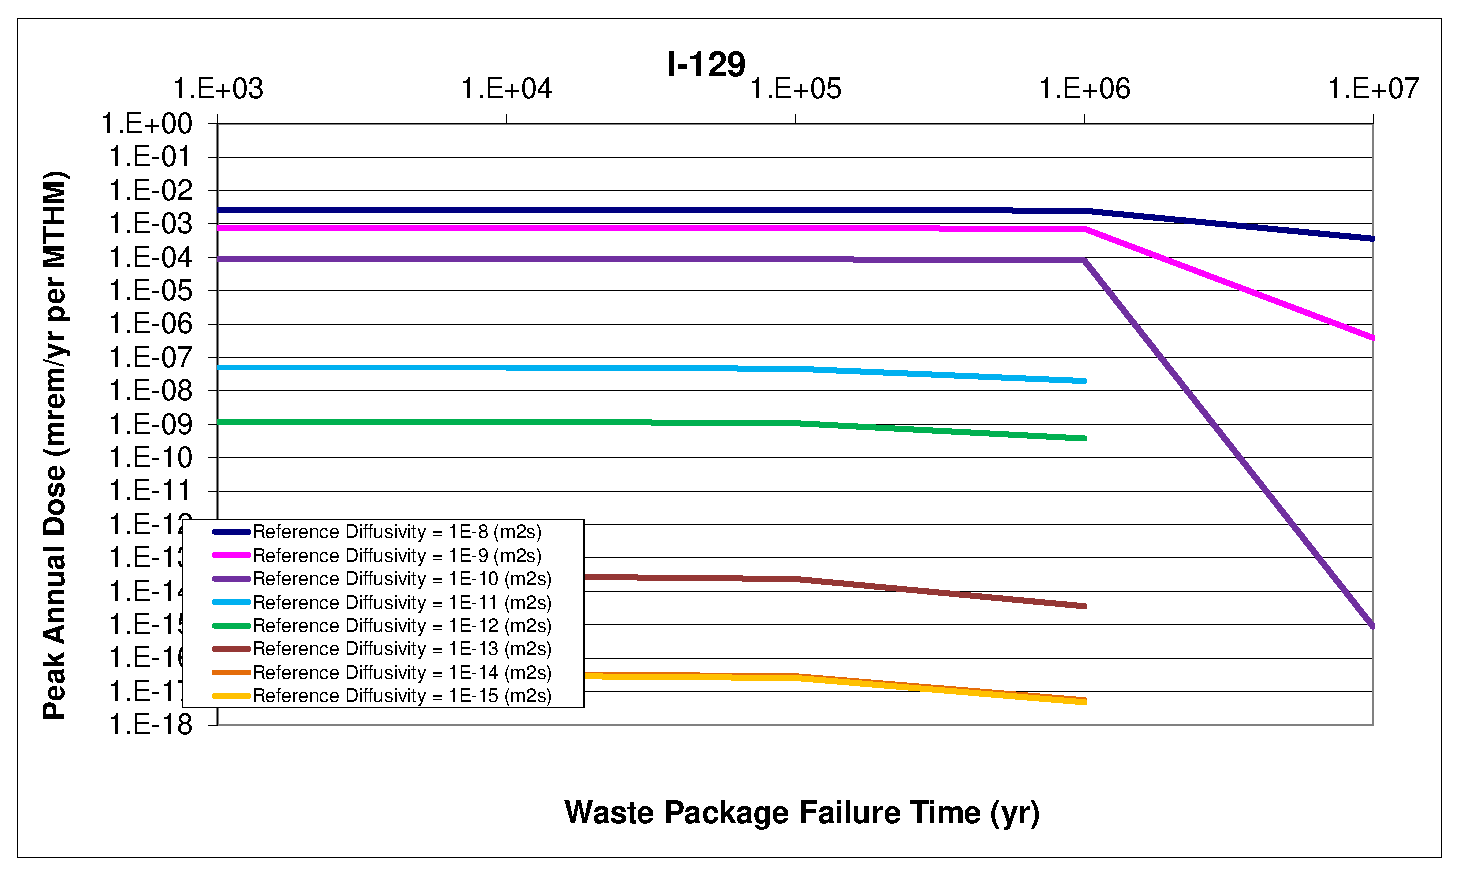
\includegraphics[width=0.8\textwidth]{WPFailExtended/I-129-WPFail.eps}
\caption{$^{129}I$ waste package failure time sensitivity. }
\label{fig:WPFailI129}
\end{figure}
\end{frame}

\begin{frame}[c]
  \frametitle{Case VI : Waste Package Failure Time and Diffusion Coefficient}

\begin{figure}[ht!]
\centering
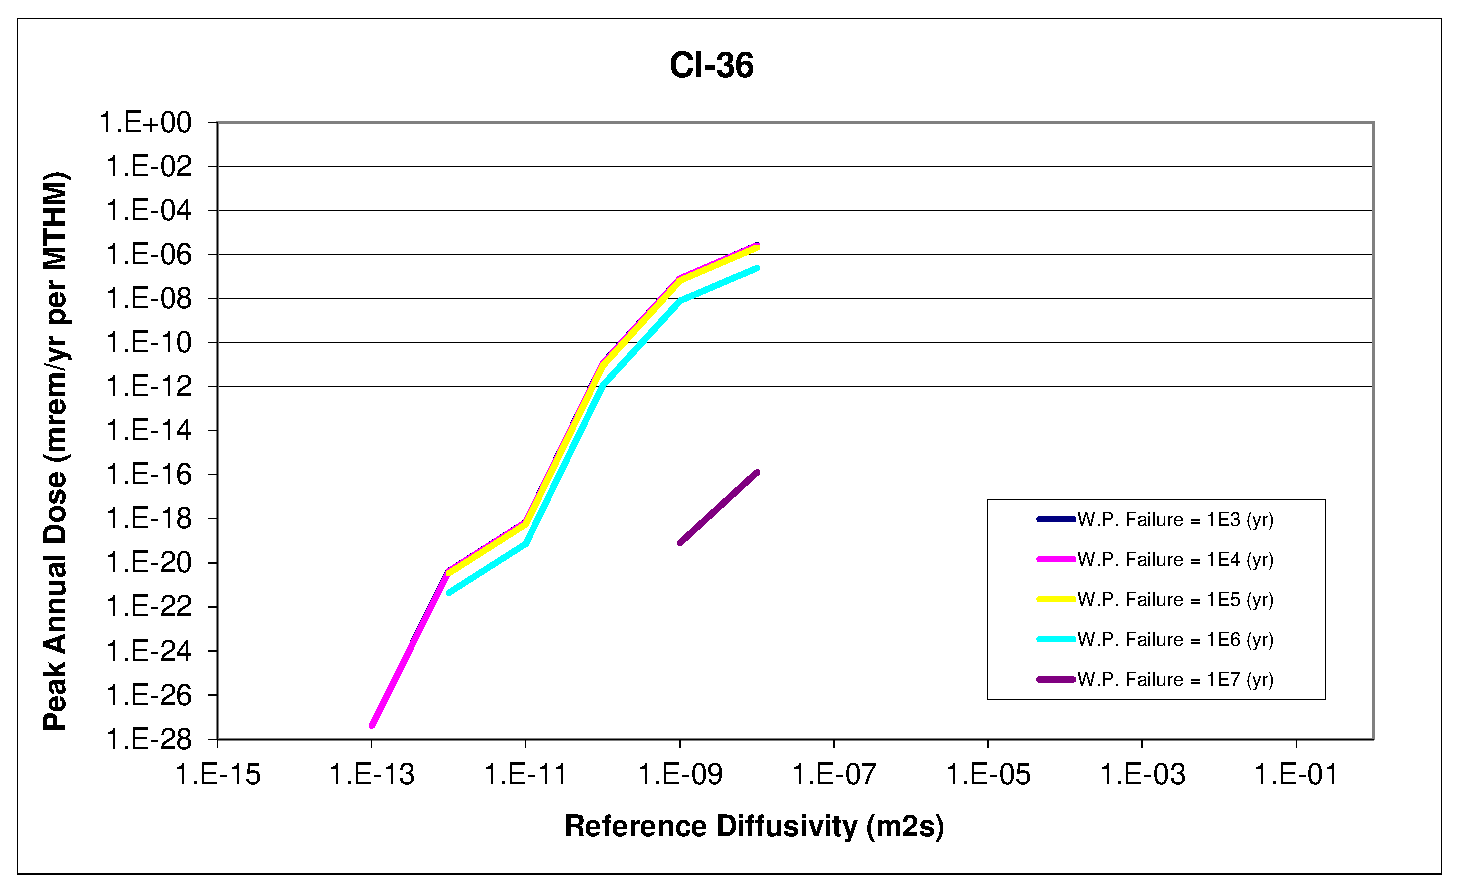
\includegraphics[width=0.8\textwidth]{WPFailExtended/Cl-36.eps}
\caption{$^{36}Cl$ waste package failure time sensitivity. }
\label{fig:WPFailCl36}
\end{figure}
\end{frame}

\begin{frame}[c]
  \frametitle{Case VI : Waste Package Failure Time and Diffusion Coefficient}

\begin{figure}[ht!]
\centering
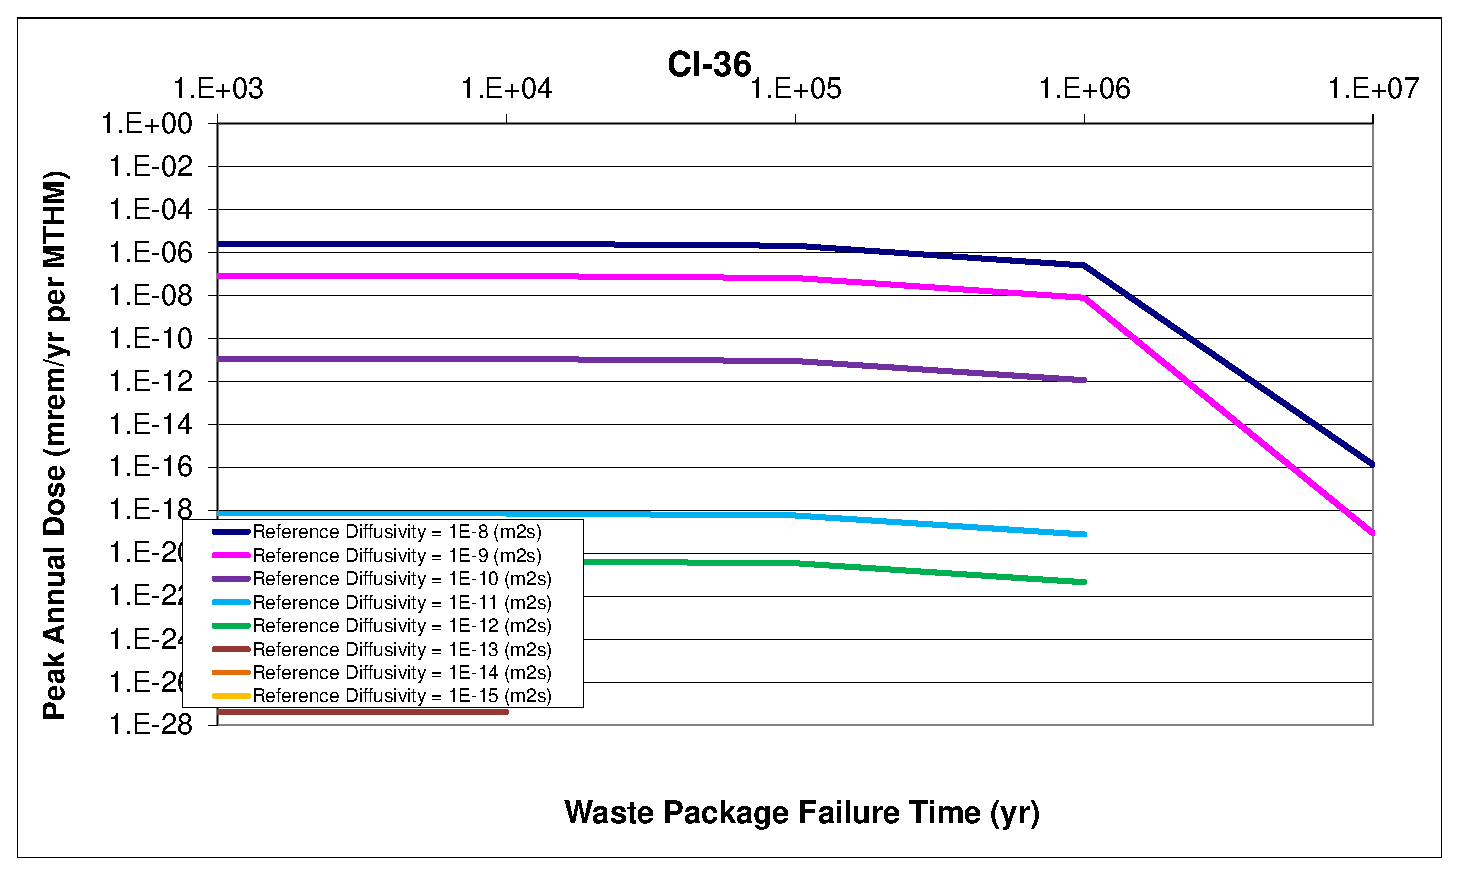
\includegraphics[width=0.8\textwidth]{WPFailExtended/Cl-36-WPFail.eps}
\caption{$^{36}Cl$ waste package failure time sensitivity. }
\label{fig:WPFailPuDaughters}
\end{figure}

\end{frame}

\begin{frame}[c]
  \frametitle{Case VI : Waste Package Failure Time and Diffusion Coefficient}
\begin{figure}[ht!]
\centering
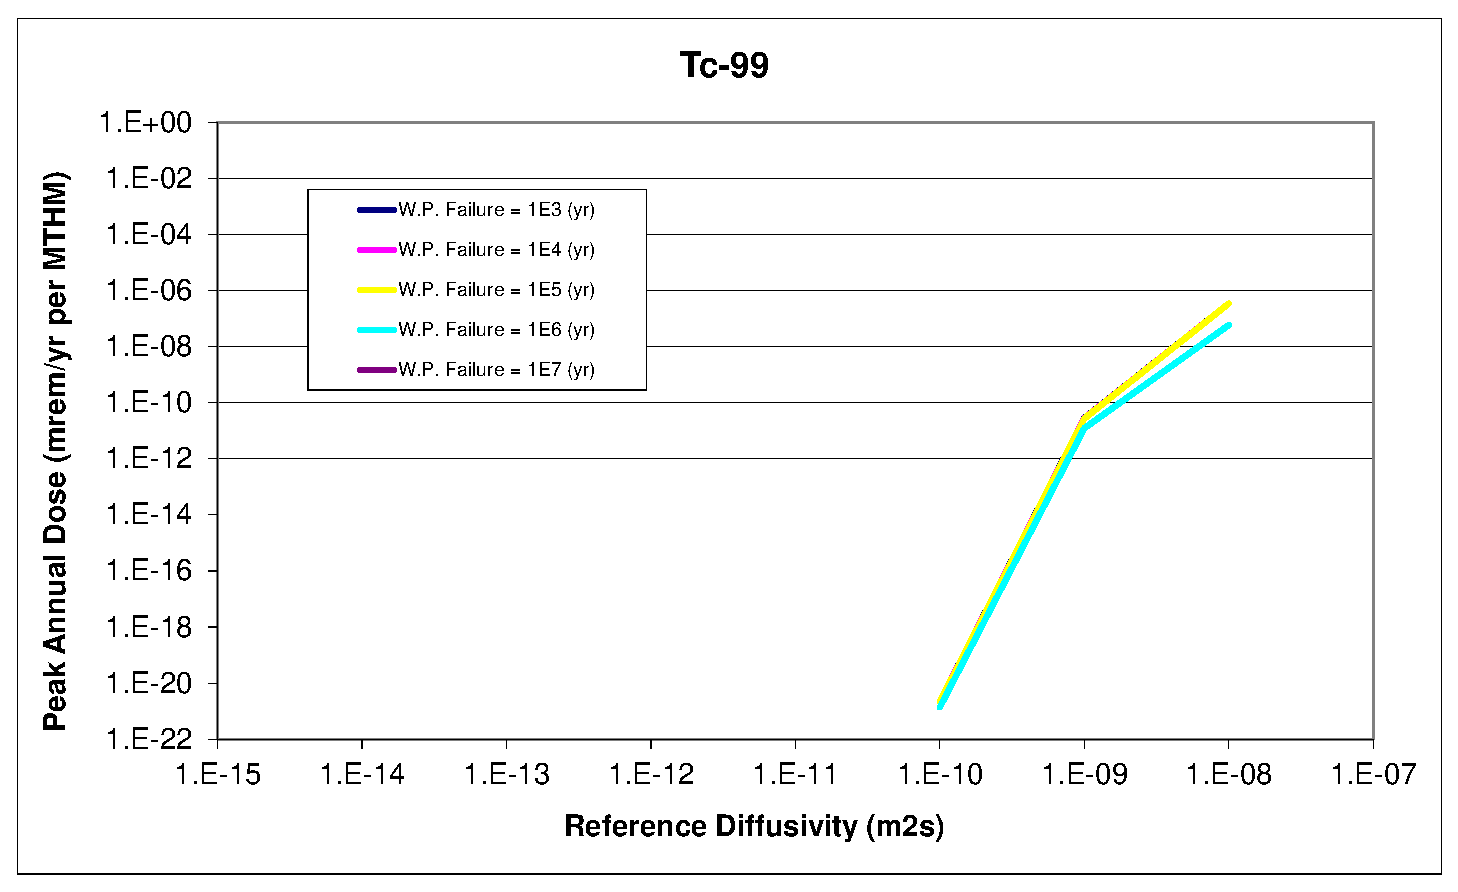
\includegraphics[width=0.8\textwidth]{WPFailExtended/Tc-99.eps}
\caption{$^{99}Tc$ waste package failure time sensitivity. }
\label{fig:WPFailTc99}
\end{figure}
\end{frame}

\begin{frame}[c]
  \frametitle{Case VI : Waste Package Failure Time and Diffusion Coefficient}

\begin{figure}[ht!]
\centering
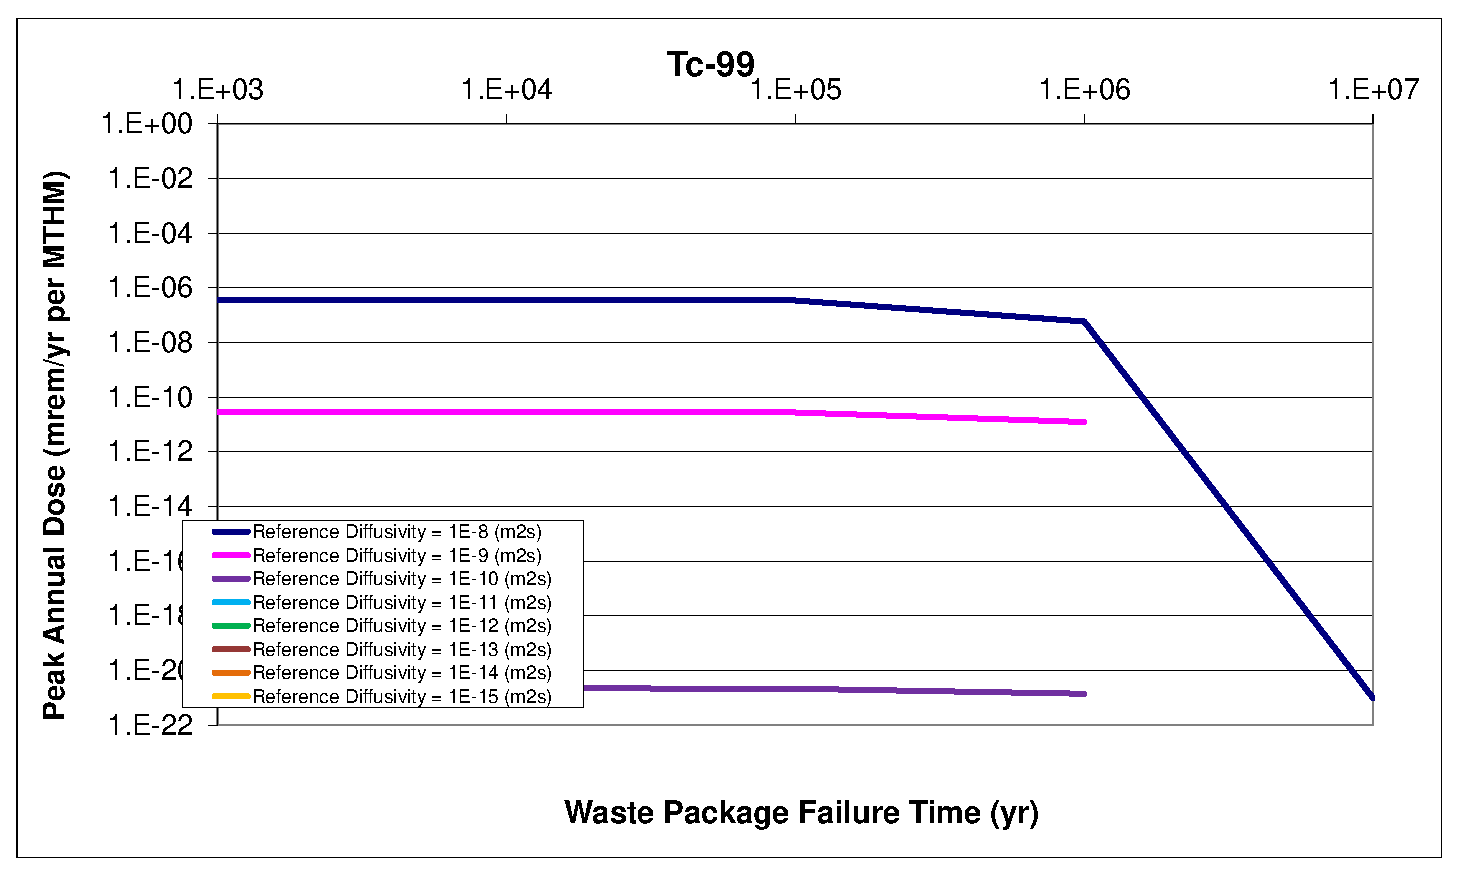
\includegraphics[width=0.8\textwidth]{WPFailExtended/Tc-99-WPFail.eps}
\caption{$^{99}Tc$ waste package failure time sensitivity. }
\label{fig:WPFailTc99}
\end{figure}
\end{frame}

\begin{frame}[c]
  \frametitle{Case VI : Waste Package Failure Time and Diffusion Coefficient}

\begin{figure}[ht!]
\centering
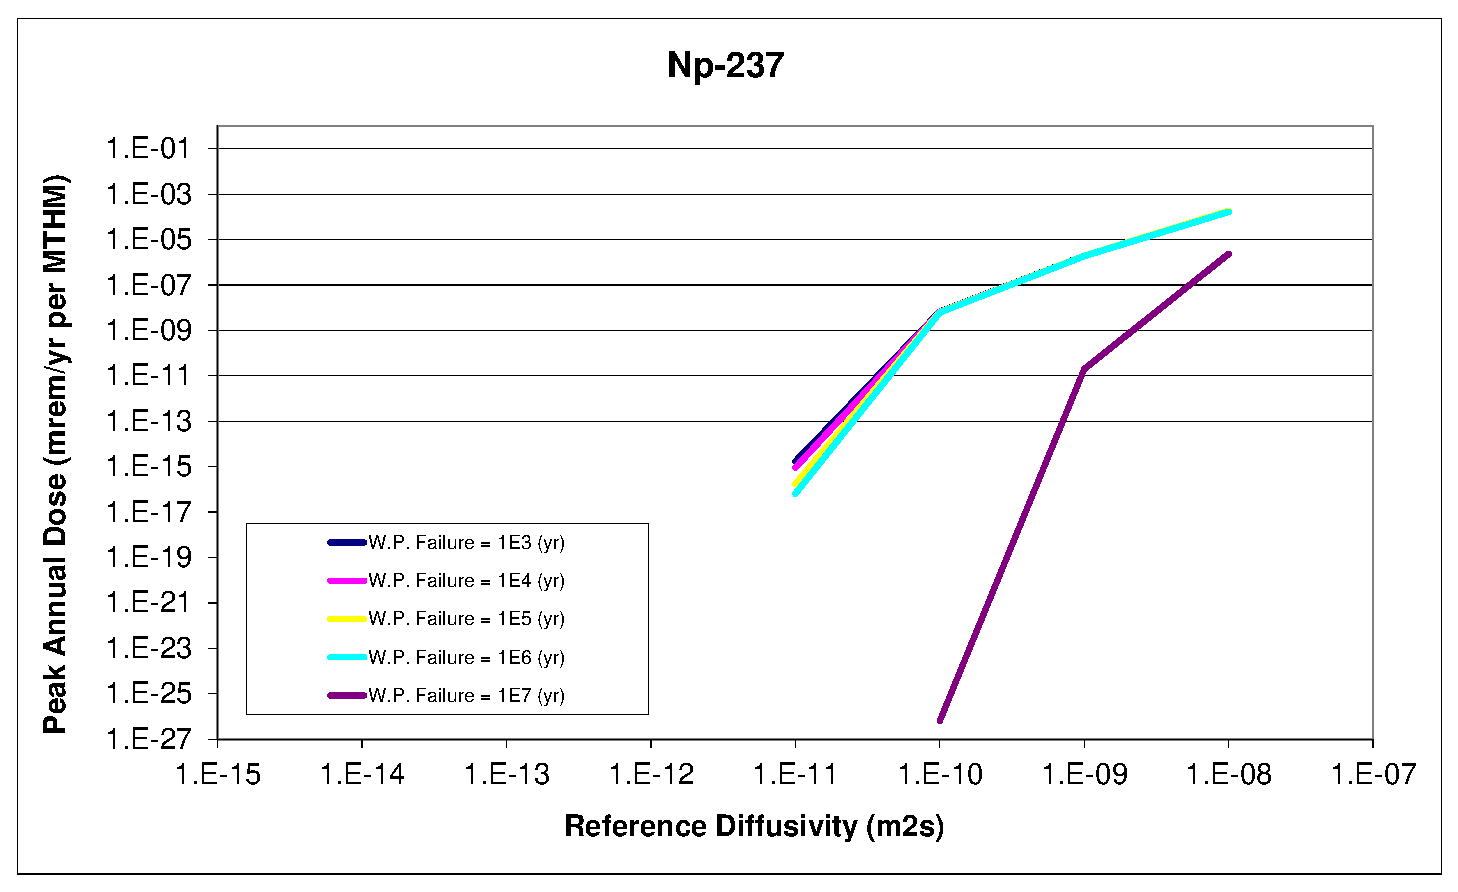
\includegraphics[width=0.8\textwidth]{WPFailExtended/Np-237.eps}
\caption{$^{237}Np$ waste package failure time sensitivity. }
\label{fig:WPFailNp237}
\end{figure}
\end{frame}

\begin{frame}[c]
  \frametitle{Case VI : Waste Package Failure Time and Diffusion Coefficient}

\begin{figure}[ht!]
\centering
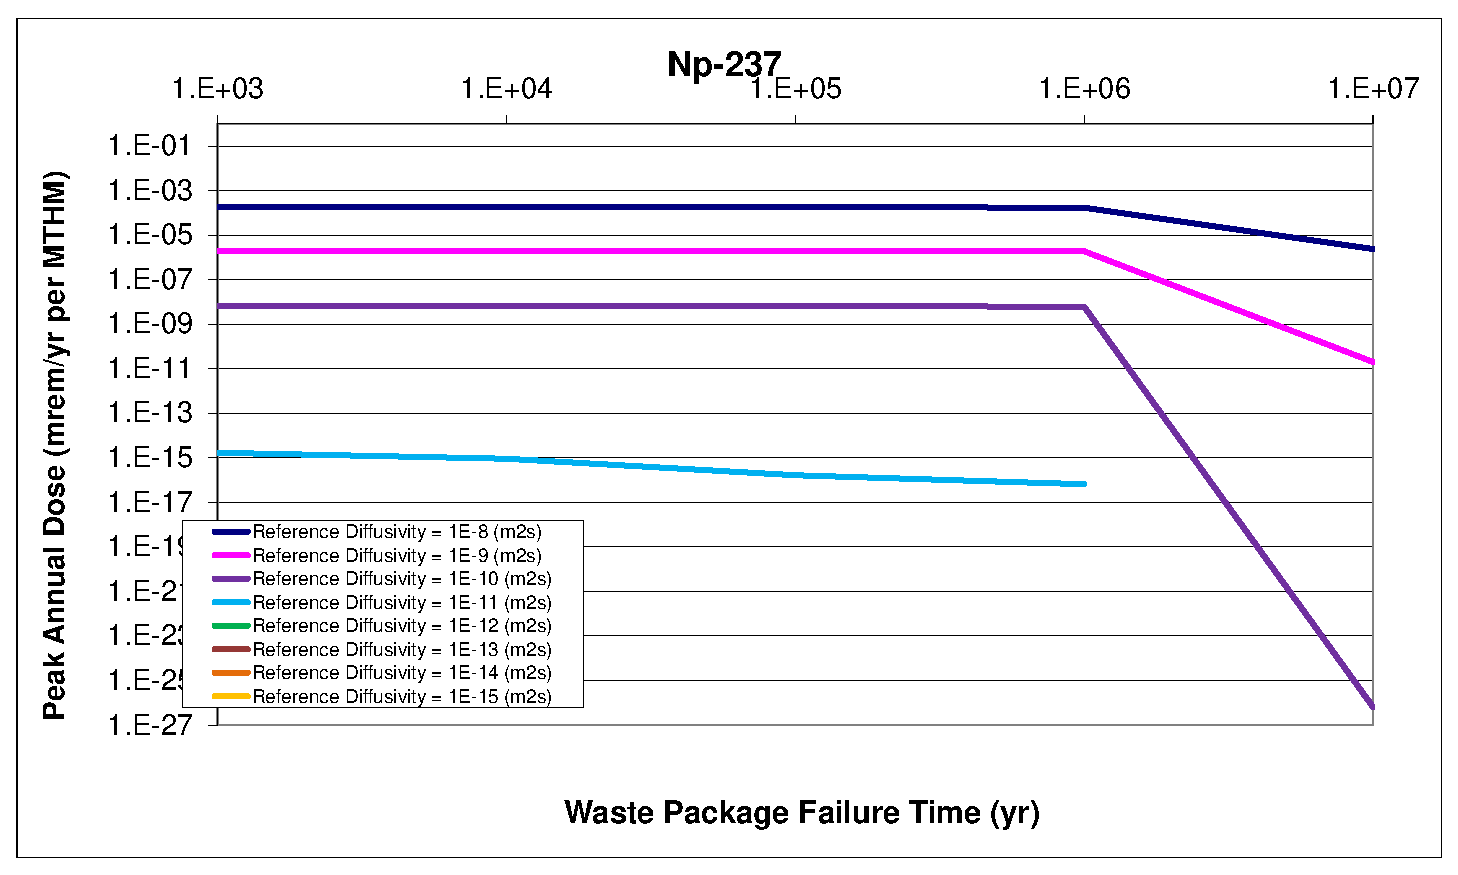
\includegraphics[width=0.8\textwidth]{WPFailExtended/Np-237-WPFail.eps}
\caption{$^{237}Np$ waste package failure time sensitivity. }
\label{fig:WPFailPuDaughters}
\end{figure}
\end{frame}

